\section{Sałatka z cieciorki z karmelizowaną cebulką}
\bigskip
\small
\begin{minipage}{0.45\textwidth}
    \noindent \textbf{Czas:} 30 minut \\
    \textbf{Poziom trudności:} łatwy
\end{minipage}
\begin{minipage}{0.45\textwidth}
    \noindent \textbf{Ilość sprzątania:} minimalna \\
    \textbf{Wymagany mysi sprzęt:} -
\end{minipage}
\normalsize
\vspace{0.5cm}

\begin{multicols}{2}

\subsection*{Składniki}
\begin{itemize}
    \item 1 puszka ciecierzycy
    \item 3 żółte cebule
    \item 1 łyżka majonezu
    \item 1 łyżka masła
    \item 1 kopiasta łyżka płatków drożdżowych nieaktywnych
    \item 1 łyżeczka startej skórki z cytryny
    \item 1 średni ząbek czosnku
    \item 0.5 łyżeczki papryki wędzonej
    \item 0.5 łyżeczki cukru (opcjonalnie)
    \item 1 płaska łyżeczka musztardy (opcjonalnie)
    \item sól i pieprz do smaku
\end{itemize}

\columnbreak

\begin{figure}[H] \centering
\fbox{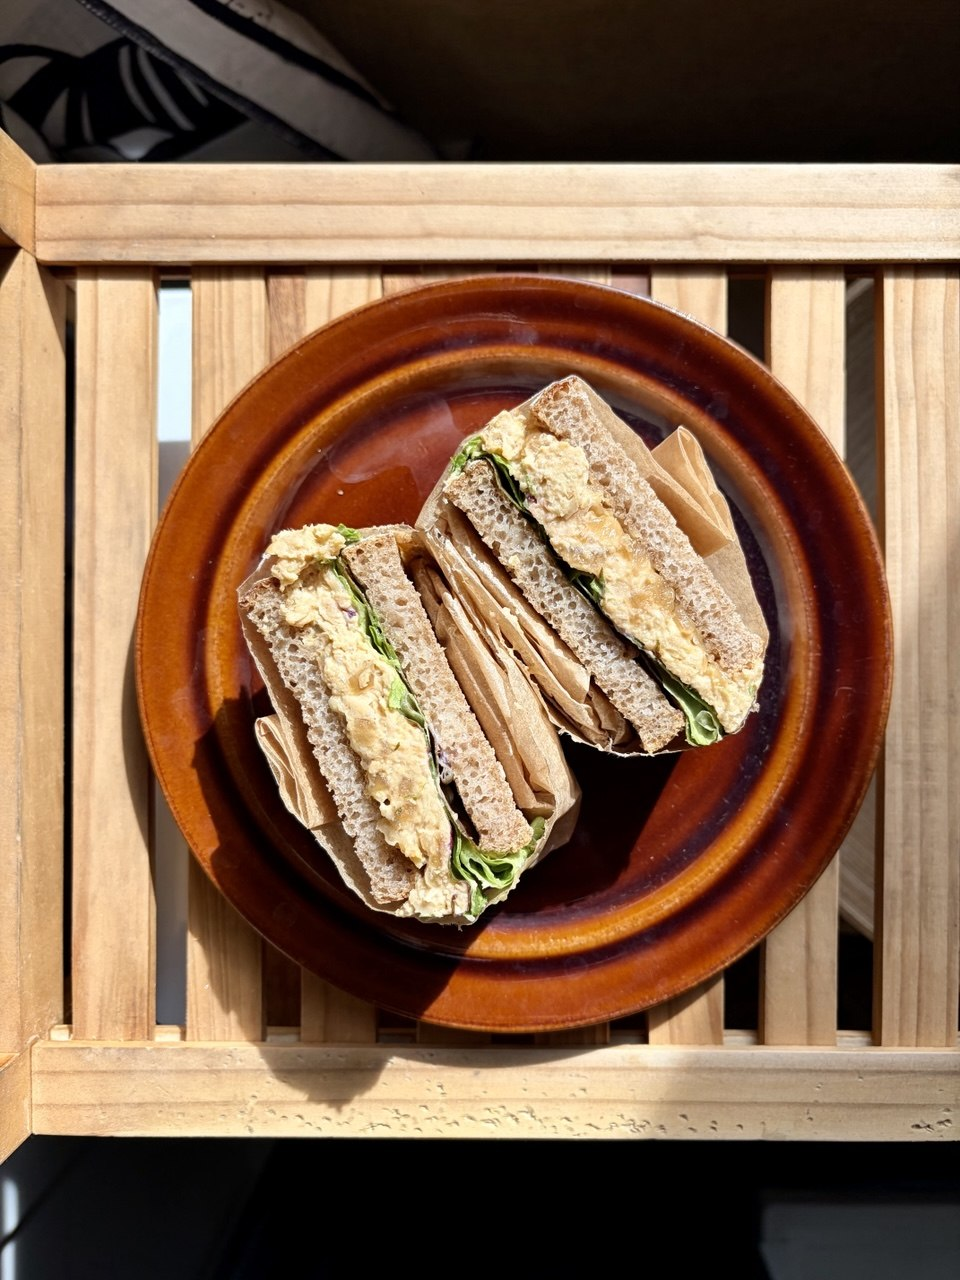
\includegraphics[width=0.35\textwidth]{images/salatka-z-cieciorki.jpg}}
\end{figure}

\end{multicols}

\vspace{0.5cm}

\subsection*{Instruktaż}
\begin{enumerate}
    \item Cebule obrać i pokroić na piórka. W średniej wielkości garnku lub patelni roztopić masło i dodać pokrojone cebule wraz ze szczodrą szczyptą soli i pieprzu oraz opcjonalnie cukrem. Smażyć \textit{cierpliwie} na \textit{bardzo małym ogniu} przez ok. 30-45 minut lub do momentu uzyskania głębokiej, bursztynowej barwy.
    \item W międzyczasie odsączyć ciecierzycę, przełożyć na talerz i rozgnieść do uzyskania pożądanej konsystencji ubijaczką do ziemniaków lub widelcem. Przełożyć ciecierzycę do miski, dodać starty ząbek czosnku i pozostałe składniki. Całość dokładnie wymieszać i doprawić solą oraz pieprzem do smaku.
    \item Doprawioną sałatkę podawać z warstwą delikatnie przestudzonej karmelizowanej cebulki.
\end{enumerate}

\vspace{0.5cm}

\small \subsection*{Propozycja podania} Na grzance lub świeżym pieczywie z chrupiącą sałatą.

\vspace{0.3cm}

\subsection*{Dodatkowe uwagi} Majonez można zastąpić jogurtem greckim.

\newpage
